\documentclass{llncs}
\usepackage[T2A]{fontenc}
\usepackage[utf8]{inputenc}
\usepackage[russian]{babel} 
\usepackage{graphicx}
\usepackage{natbib}
\usepackage{amsfonts}
\usepackage{alltt}

\title{Распознавание текста на основе скелетного представления толстых линий и сверточных сетей }

\author{Соломатин А.А.}
\institute{Московский физико-технический институт (Государственный университет) \\ 
\email{solomatin.aa@phystech.edu}}

\begin{document}

\maketitle

\begin{abstract}
Задача распознавания символа на картинке является чрезвычайно распространенной задачей машинного обучения. В связи с этим существует несколько основных подходов к решению. В первом методе мы используем сверточные нейросети небольшой глубины для анализа изображения. В другом методе мы представляем символ в виде графа. Из скелета этого графа строится вектор признаков, который затем обрабатывается нейросетью. Также приводится сравнение точности классификации этих алгоритмов на датасете MNIST.
\end{abstract}

\textit{Ключевые слова: сверточные нейронные сети, CNN, распознавание символов, скелетное представление, Graph embedding}

\section{Введение}

Распознавание текста на изображении это классическая задача компьютерного зрения в машинном обучении. В данной работе мы имеем дело с изображениями символов. Регулярно появляются работы, призванные улучшить точность классификации. Основным подходом к решению является использование сверточных слоев в нейронных сетях, описанное в~\cite{cnn_1}~\cite{cnn_2}. Для улучшения качества нам предложено использовать векторное представление изображения вместо растрового. Векторное представление получается из графого представления путем построения скелетов символов. 

При скелетизации внутренности символов заполняются кругами, центры которых являются вершинами графа и соединяются его ребрами. На сегодняшний день существует много исследований на тему скелетизации. В работе~\cite{graphs_gen} описывается математический аппарат для генерации рукописного текста с помощью жирных линий, а в работе~\cite{graphs_shape_comp} сравниваются формы растровых изображений при помощи скелетизации. В тоже время разработаны и альтернативные подходы, описанные в статье~\cite{graphs_alt_method}. 

Граф, получаемый после скелетизации, не может быть подан на вход нейронной сети. Поэтому нам необходимо векторизовать граф с помощью его эмбеддинга. 
Для оценки качества работы алгоритма предлагается использовать датасет MNIST. Он состоит из рукописных цифр и использовался для валидации во многих работах, таких как~\cite{mnist_sample1},~\cite{mnist_sample2},~\cite{mnist_sample3}.

\section{Постановка задачи}

Введем следующие обозначения: 
\begin{itemize}
\item $\mathbb{I}$ - множество пар черно-белых бинаризованных изображений и сопоставленных им меток, символов из алфавита $\mathbb{A}$. На изображении содержится только один символ. 

Пусть функция $a: \mathbb{I} \rightarrow \mathbb{A}$ однозначно сопоставляет каждому изображению из $\mathbb{I}$ его метку класса.

\item $\mathbb{G}$ - пространство графов скелетных представлений символов. Под скелетным представлением здесь подразумевается неориентированный граф, каждой вершине которого сопоставлено некоторое число, называемое радиусом.

Функция $g: \mathbb{I} \rightarrow \mathbb{G}$ однозначно сопоставляет каждому изображению из $\mathbb{I}$ его скелетное представление. В данной работе в качестве такой функции используется алгоритм, описанный в работе~\cite{cnn_1}.

\item $\mathbb{V}$ - векторное пространство. Будем считать что граф представим в векторном виде сюрьективным преобразованием $v: \mathbb{G} \rightarrow \mathbb{V}$

\item $\mathbb{F}$ - пространство признаков графов, описывающих скелетное представление символов.

Функция $f: \mathbb{I} \rightarrow \mathbb{G}$ однозначно сопоставляет каждому элементу из $\mathbb{G}$ множество его признаков.

\item Необходимо также ввести преобразование, которое вычисляет признаки графа. $t: \mathbb{G} \rightarrow \mathbb{F}$

\item $\mathbb{Y}$ - пространство меток (номеров символов в алфавите).
\end{itemize}

Тогда, задачей данного исследования является нахождение функций:$y: \mathbb{I} \rightarrow \mathbb{Y}$, $h: \mathbb{F} \rightarrow \mathbb{Y}$, $d: \mathbb{V} \rightarrow \mathbb{Y}$,
 
Минимизируется функционал, который вычисляет функцию ошибки, L - cross entropy loss, для различных функций.

\section{Решения}
\subsection{Неронная сеть}
В качестве первого базового алгоритма было решено использовать сверточную нейронную сеть. Она написана с использованием библиотеки keras:
\begin{alltt}
model = Sequential()
model.add(Conv2D(30, (5, 5), 
    input_shape=(1, 28, 28), 
    activation='relu'))
model.add(MaxPooling2D(pool_size=(2, 2)))
model.add(Conv2D(15, (3, 3), activation='relu'))
model.add(MaxPooling2D(pool_size=(2, 2)))
model.add(Dropout(0.2))
    
model.add(Flatten())
model.add(Dense(128, activation='relu'))
model.add(Dense(50, activation='relu'))
model.add(Dense(num_classes, activation='softmax'))

model.compile(loss = keras.losses.categorical_crossentropy, 
                  optimizer = keras.optimizers.Adadelta(), 
                  metrics=['accuracy', f1])
\end{alltt}

\subsection{Градиентный бустинг}
В качестве второй базовой модели был использован LightGBM Classifier, который обучился на признаках из скелетного представления. Данный алгоритм основывается на градиентном бустинге над деревьями решений.

\subsection{Смешанная модель}
Смешанная модель, работающая с изображением и признаками, полученными с помощью градиентного бустинга. Признаки добав-
ляются после прохождения картинкой свёрточных
фильтров и преобразования в одномерный тензор. Нейронная сеть написана с помощью библиотеки keras:
\begin{alltt}
model_cnn_input = Input((28, 28, 1))
cnn = Conv2D(30, (3, 3), activation='relu', input_shape = input_shape_cnn)(model_cnn_input)
cnn = Conv2D(60, (3, 3), activation='relu')(cnn)
cnn = MaxPooling2D(pool_size=(2, 2))(cnn)
cnn = BatchNormalization()(cnn) 
cnn = Activation('relu')(cnn)
cnn = Dropout(0.2)(cnn)
cnn = MaxPooling2D(pool_size=(2, 2))(cnn)

cnn = Flatten()(cnn)
cnn = Dense(128, activation='relu')(cnn)

features_input = Input(input_dim_skelet)
features_layer1 = Dense(32, input_dim=input_dim_skelet)(features_input)

merged = Concatenate()([cnn, features_layer1])
layer1 = Dropout(0.5)(merged)
output_layer = Dense(num_classes, activation='softmax')(layer1)

model = Model(inputs=[model_cnn_input, features_input], outputs=output_layer)
model.compile(loss="categorical_crossentropy",
              optimizer="adam",
              metrics=['accuracy', f1])
\end{alltt}

\section{Планирование эксперимента}
\subsection{Датасет}
В исследовании используется набор изображений с рукописным текстом MNIST.
К каждому изображению построен его скелетный граф, методом, описанным в~\cite{graphs_gen}. Для скелетизации, картинка должна быть бинаризованной. В этих данных бинаризация была следующая: все пиксели, кроме черных(то есть > 0 в нотации цветов от 0 до 255), обращаются в белый. Вершины графа описываются четыремя числами: координатами по оси абсцисс, ординат, степень вершины (она может быть от 1 до 3, таков алгоритм построения скелета), радиальная функция в этой точке, или же, радиус вписанной в фигуру окружности в этой точке.

\subsection{Неронная сеть}
Модель на вход принимает черно-белые изображения размером 28 на 28. На выходе дает вероятности принадлежности к каждому из классов. Для обучения нейросети было произведено разбиение выборки на обучение,
валидацию и тестирование в соотношении 600000:5000:5000. Веса оптимизи-
ровались алгоритмом AdaDelta.

\subsection{Градиентный бустинг}
Для обучения и предсказания использовалась модель LGBMClassifier.
На вход модель принимала различного рода статистики, посчитанные на скелетном представлении изображения.
Используемые статистики:
\begin{itemize}
    \item Количество вершин в скелетном представлении
    \item Среднее значение среди всех чисел, как представленных в описании графа, так и по каждой из 8 подряд идущих чисел
    \item Сумма как всех чисел, представленных в описании графа, так и по каждой из 8 подряд идущих чисел
    \item Дисперсия как среди всех чисел, представленных в описании графа, так и по каждой из 8 подряд идущих чисел
    \item Разность между максимальным и минимальным числом как среди всех чисел, представленных в описании графа, так и по каждой из 8 подряд идущих чисел
    \item Перцентили от 0 до 1 с шагом 0.1 как среди всех чисел, представленных в описании графа, так и по каждой из 8 подряд идущих чисел
    \item Для каждой из четырёх категорий самое частое значение и сколько раз оно встретилось
\end{itemize}

\section{Анализ ошибок}
Ниже приведены графики функции потери, а так же точности
и F1 метрики на валидации Для первого эксперимента со сверточной нейросетью и третьего эксперимента со сверточной нейросетью и признаками из второго эксперимента.

\begin{wrapfigure}
\centering
\caption{Анализ функции ошибки и score обычной сверточной нейронной сети\label{overflow}}
\begin{center}
    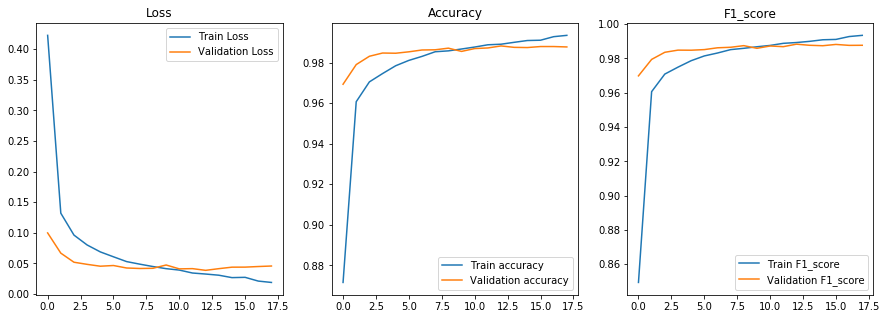
\includegraphics[width=90mm]{loss_1.jpg}}
  \end{center}
\end{wrapfigure}


\begin{wrapfigure}
\centering
\caption{Анализ функции ошибки и score в смешанном эксперименте\label{overflow}}
\begin{center}
    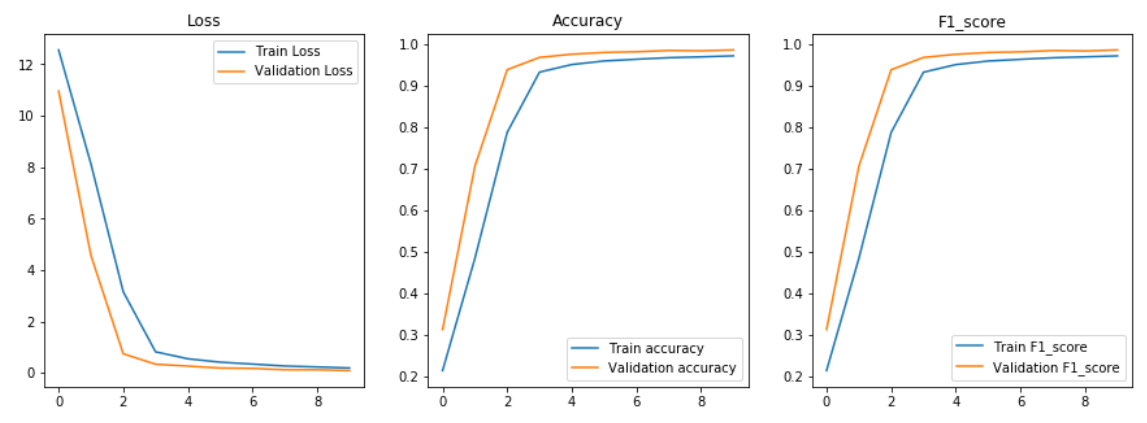
\includegraphics[width=90mm]{Graph_mixed.png}
  \end{center}
\end{wrapfigure}

\section{Анализ структуры модели}
\subsection{Неронная сеть}
Путем перебора была подобрана финальная конфигурация фильтров свёрточных слоёв.
\begin{wrapfigure}
\centering
\caption{Конфигурация слоев\label{overflow}}
\begin{center}
    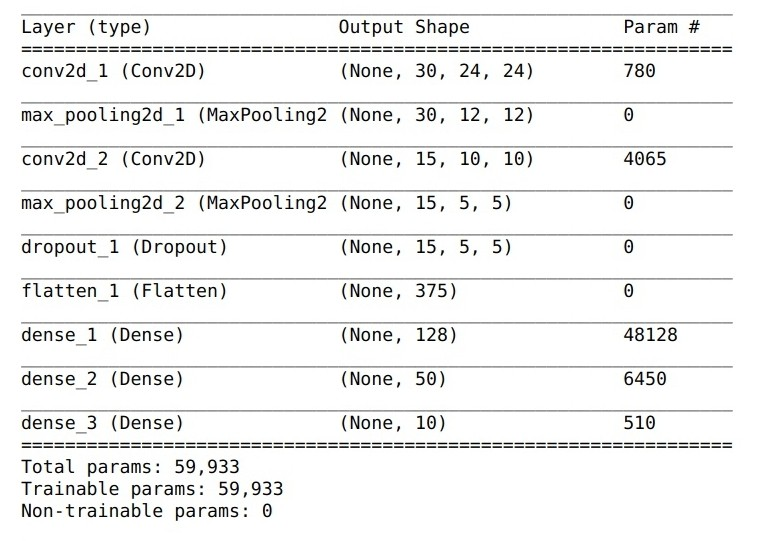
\includegraphics[width=90mm]{model_1.jpg}}
  \end{center}
\end{wrapfigure}

\subsection{Градиентный бустинг}
После построения признаков были проведенны эксперименты по изменению параметров модели. Количество листьев было увеличено до 110. learning_rate был уменьшен, а n_estimators увеличены в 7 раз.

\subsection{Смешанная модель}
Итоговая структура комбинированной нейронной сети:
\begin{wrapfigure}
\centering
\caption{Конфигурация слоев\label{overflow}}
\begin{center}
    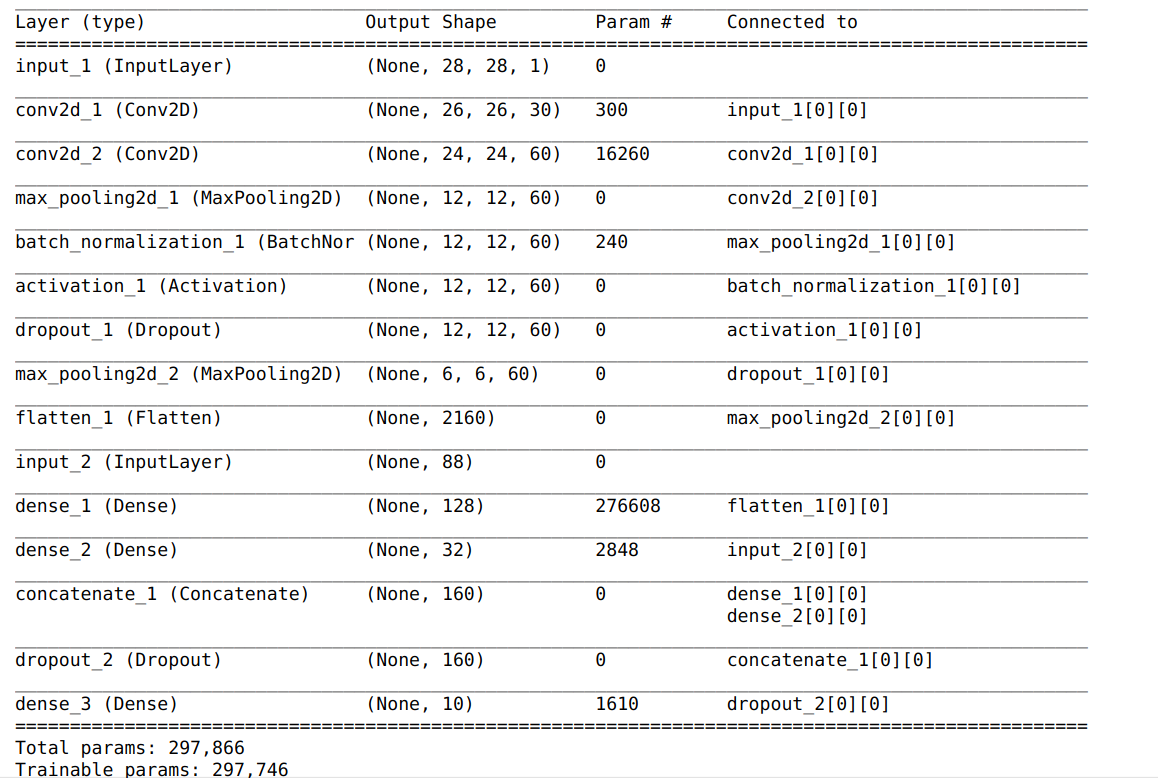
\includegraphics[width=90mm]{model_2.png}}
  \end{center}
\end{wrapfigure}

\section{Выбор модели}
\begin{wraptable}
\label{tabular:timesandtenses}
\begin{center}
\begin{tabular}{ccc}
Модель & Accuracy & F1-score \\
Нейросеть: & \textbf{0.9813} & \textbf{0.9816} \\
LightGBM: & \textbf{0.9319} & \textbf{0.9309} \\
Смешанная модель & \textbf{0.9849} & \textbf{0.9851} \\
\end{tabular}
\end{center}
\end{wraptable}

\section{Результат работы}
В результате приведенного исследования было рассмотренно несколько подходов к решению задачи распознования символов на изображении. Один из методов использовал сверточные сети для классификации изображений. Другой метод заключался в анализе графовых струтур с помощью скелетного представления, полученных по изображению. Так же были приведены сравнения точности этих подходов и архитектур на датасетах MNIST.

\begin{thebibliography}{1}

\bibitem{cnn_1}
	\BibAuthor{LeCun Y. et al.}
	 Convolutional networks for images, speech, and time series //The handbook of brain theory and neural networks. – 1995. – Т. 3361. – №. 10. – С. 1995.
	 
\bibitem{cnn_2}
	\BibAuthor{Ciresan D. C. et al.}
 	Convolutional neural network committees for handwritten character classification //Document Analysis and Recognition (ICDAR), 2011 International Conference on. – IEEE, 2011. – С. 1135-1139.
 
\bibitem{graphs_gen}
	\BibAuthor{Клименко С. В., Местецкий Л. М., Семенов А. Б.}
	 Моделирование рукописного шрифта с помощью жирных линий //Труды. – 2006. – Т. 16.

\bibitem{graphs_shape_comp}
	\BibAuthor{Кушнир О. и др.}
	 Сравнение формы бинарных растровых изображений на основе скелетизации //Машинное обучение и анализ данных. – 2012. – Т. 1. – №. 3. – С. 255-263.
	 
\bibitem{graphs_alt_method}
	\BibAuthor{Масалович А., Местецкий Л.}
	 Распрямление текстовых строк на основе непрерывного гранично-скелетного представления изображений //Труды Международной конференции «Графикон», Новосибирск.–2006.–4 c.

\bibitem{mnist_original}
	\BibAuthor{LeCun Y., Cortes C., Burges C. J.}
	MNIST handwritten digit database //
	Available: 
	 \BibUrl{http://yann. lecun. com/exdb/mnist}. – 2010. – Т. 2.

\bibitem{mnist_sample1}
	\BibAuthor{Zhu D. et al.}
	 Negative Log Likelihood Ratio Loss for Deep Neural Network Classification //arXiv preprint arXiv:1804.10690. – 2018.
	 
\bibitem{mnist_sample2}
	\BibAuthor{Nair P., Doshi R., Keselj S.}
	Pushing the limits of capsule networks //Technical note. – 2018.

\bibitem{mnist_sample3}
	\BibAuthor{Hsieh P. C., Chen C. P.}
	 Multi-task Learning on MNIST Image Datasets. – 2018.

\end{thebibliography}

\end{document}
